\begin{frame}{Simulation of the Langevin equation}
Two possible approximation methods.
  		\begin{block}{Overdamped}
  	  		\begin{equation*}
  	  		\dot{v} = F - \nabla U - \gamma v + \sqrt{2T\gamma}\xi_t
  	  		\end{equation*}
  	  	\end{block}
  	  	\begin{itemize}
  	  	 \item This is the most general method
  	  	\end{itemize}
  	  	\begin{block}{ Underdamped}
  	  		  			\begin{equation*}\label{eqn:overdamped}
  	  		  			\gamma v_f = F - \nabla U + \sqrt{2T\gamma}\xi_t
  	  		  			\end{equation*}
  	  		  			\begin{itemize}
  	  		  			\item Particle reaches terminal velocity after each step
  	  		  			\end{itemize}
  	  	\end{block}
\end{frame}


\begin{frame}{Results}
The result for both methods gave the same numerical result.
  \vspace{0cm}
       
        	  	\begin{minipage}{0.49\textwidth}
        	  	\begin{block}{}
        	  				\vspace{-1.7cm}
        	  	     	  	\begin{figure}
        	  	     	  	      	  \centering
        	  	     	  	      	  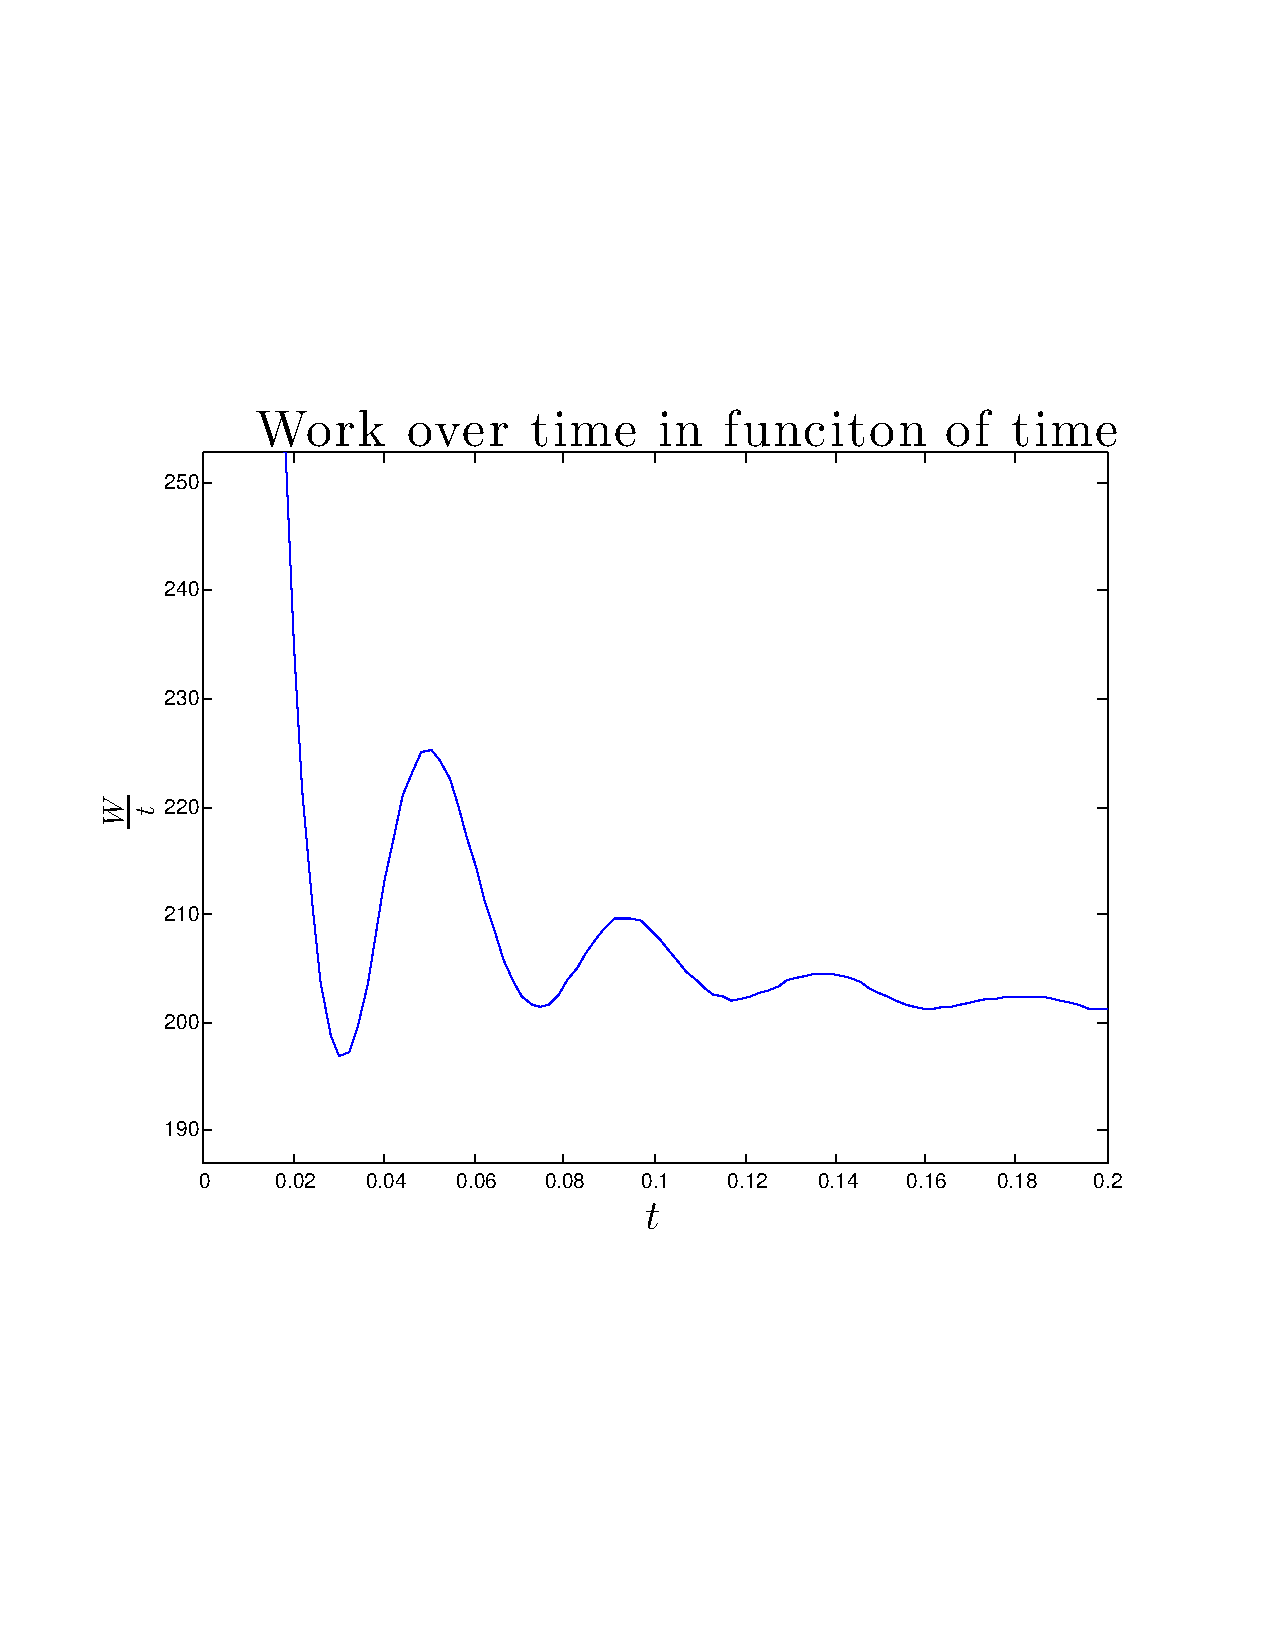
\includegraphics[width=\textwidth]{../src/plot/langevin/workOverTimeInFunctionOfTimePotential2.pdf}
        	  	     	  	 \end{figure}
        	  	\end{block}
        	  	\end{minipage}
        	  	\begin{minipage}{0.49\textwidth}
        	  			\begin{block}{}
        	  			\vspace{-1.7cm}
        	  				\begin{figure}
        	  						\centering
        	  						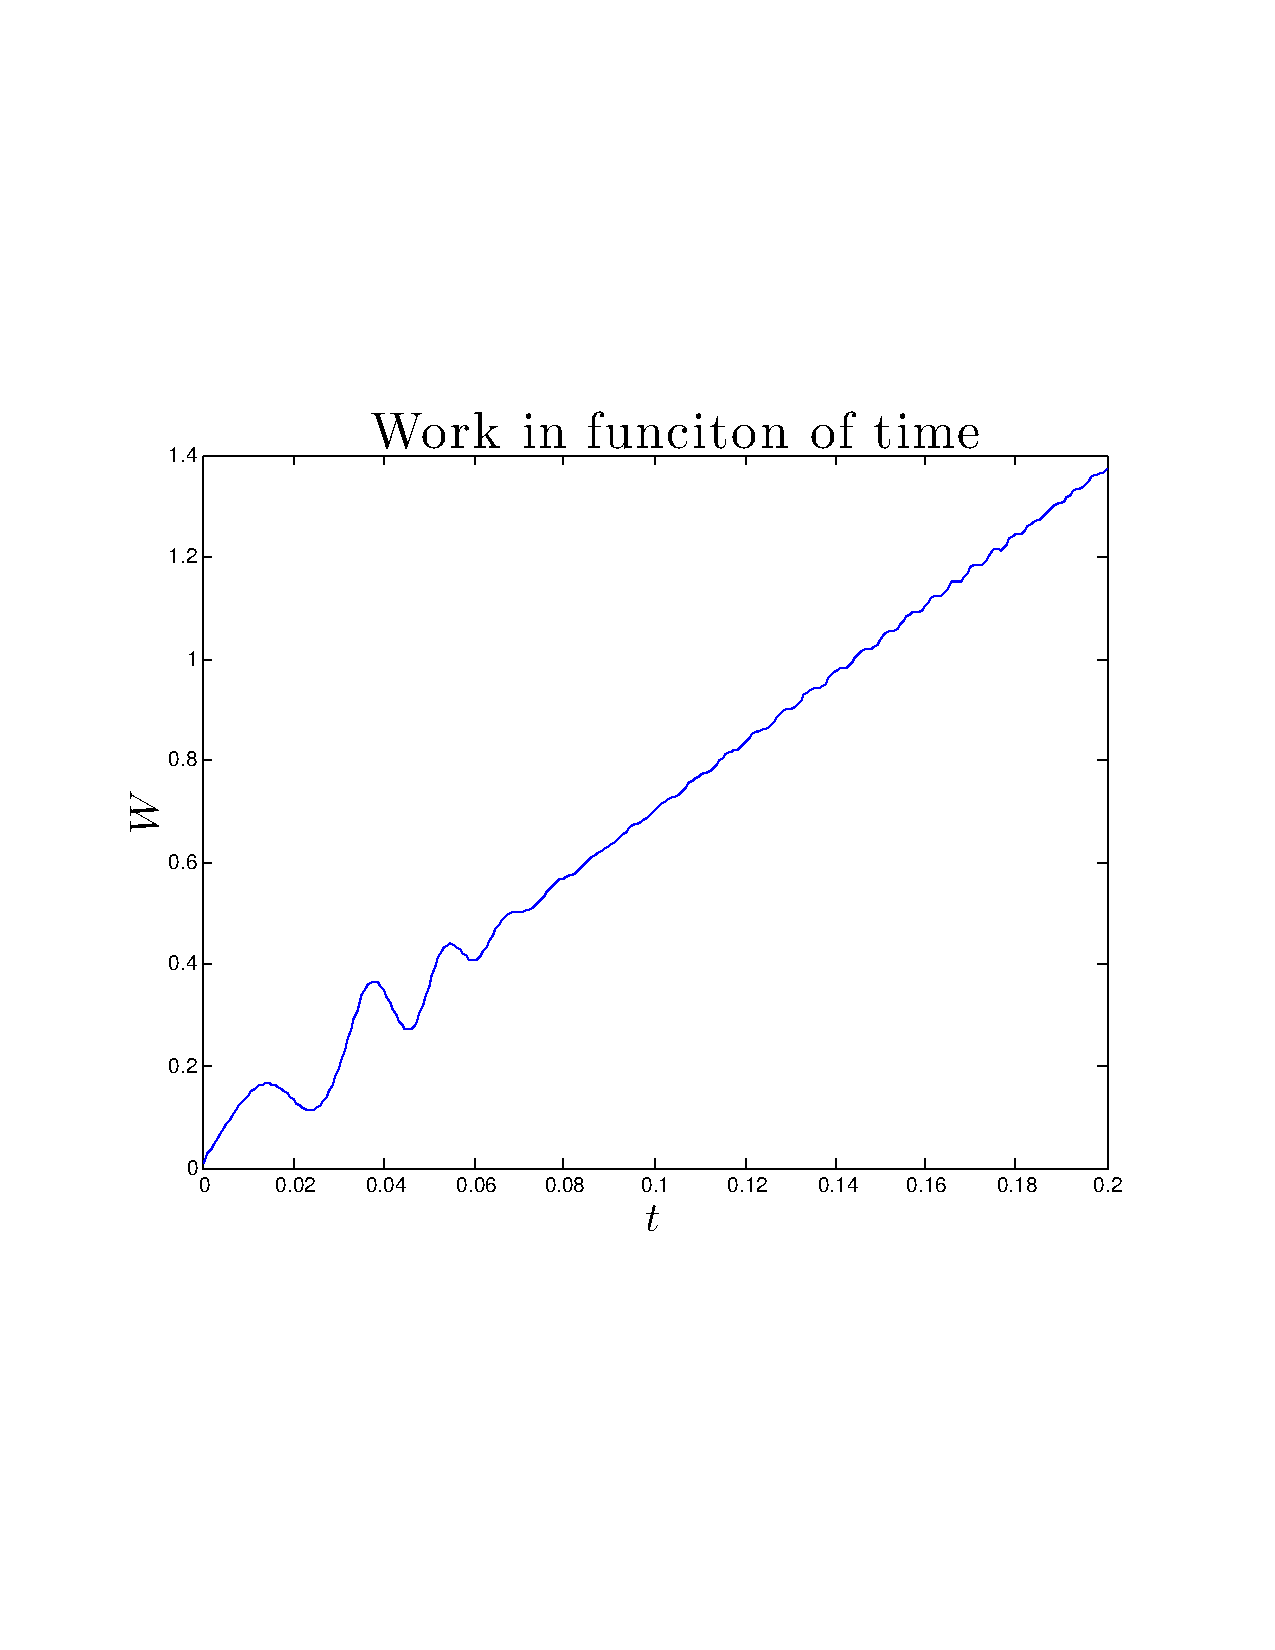
\includegraphics[width=\textwidth]{../src/plot/langevin/workInFunctionOfTimeUnerDamped.pdf}
        	  					\end{figure}
        	  		  	\end{block}
        	  	\end{minipage}
        	  	
\end{frame}
